\documentclass{article}

\usepackage{arxiv}

\usepackage{authblk}
\usepackage[utf8]{inputenc} % allow utf-8 input
\usepackage[T1]{fontenc}    % use 8-bit T1 fonts
\usepackage{hyperref}       % hyperlinks
\usepackage{cleveref}
\usepackage{url}            % simple URL typesetting
\usepackage{booktabs}       % professional-quality tables
\usepackage{amsfonts}       % blackboard math symbols
\usepackage{nicefrac}       % compact symbols for 1/2, etc.
\usepackage{microtype}      % microtypography
\usepackage{lipsum}		% Can be removed after putting your text content
\usepackage{graphicx}
\usepackage{doi}
\usepackage{xcolor}
\usepackage[english=american,autostyle=true,autopunct,csdisplay]{csquotes}

\usepackage[cache=false,newfloat=true]{minted}
\usepackage{float} % to use \begin{listing}[H]
\usemintedstyle{friendly}
\setminted[toml]{numbersep=5pt, frame=lines, framesep=2mm, gobble=0}
\setminted[ini]{numbersep=5pt, frame=lines, framesep=2mm, gobble=0}
%\setminted[json]{numbersep=5pt, frame=lines, framesep=2mm, gobble=0}
\setminted[python]{numbersep=5pt, frame=lines, framesep=2mm, gobble=0, linenos}
\setminted{frame=single,framesep=10pt}
%\BeforeBeginEnvironment{minted}{\vspace{-0.2cm}}
%\AfterEndEnvironment{minted}{\vspace{-0.2cm}}
\usepackage{caption}
\captionsetup[listing]{skip=-4pt}

\usepackage{subcaption}

\usepackage{tikz}
\usetikzlibrary{calc,positioning,shapes.geometric,backgrounds,fit,shadows.blur,arrows.meta}

\usepackage[backend=biber,sorting=none,citestyle=numeric-comp]{biblatex}
\addbibresource{references.bib}

\newcommand{\chioz}{\ensuremath{\widetilde{\chi}_{1}^{0}}}
\newcommand{\chiopm}{\ensuremath{\widetilde{\chi}_{1}^{\pm}}}
\newcommand{\chitpm}{\ensuremath{\widetilde{\chi}_{2}^{\pm}}}
\newcommand{\chitz}{\ensuremath{\widetilde{\chi}_{2}^{0}}}
\newcommand{\chithz}{\ensuremath{\widetilde{\chi}_{3}^{0}}}
\newcommand{\slepton}{\ensuremath{\widetilde{\ell}}}
\newcommand{\met}{\ensuremath{E_{\mathrm{T}}^{\mathrm{miss}}}}
\newcommand{\mapyde}{\texttt{mapyde}}
\newcommand{\simpleanalysis}{\texttt{SimpleAnalysis}}
\newcommand{\madgraph}{\textsc{MadGraph}}
\newcommand{\madspin}{\textsc{MadSpin}}
\newcommand{\pythia}{\textsc{Pythia}}
\newcommand{\delphes}{\textsc{Delphes}}
\newcommand{\pyhf}{\texttt{pyhf}}
\newcommand{\musig}{\ensuremath{\mu_{\mathrm{sig}}}}
\newcommand{\hepdata}{\texttt{HEPData}}
\newcommand{\hepmc}{\textsc{hepmc}}
\newcommand{\pt}{\ensuremath{p_{\mathrm{T}}}}
\newcommand{\easyscanhep}{\textsc{EasyScan\_HEP}}
\newcommand{\spheno}{\textsc{Spheno}}
\newcommand{\feynhiggs}{\textsc{FeynHiggs}}
\newcommand{\micromegas}{\textsc{MicrOMEGAS}}
\newcommand{\superiso}{\textsc{SuperIso}}
\newcommand{\gmtwocalc}{\textsc{GM2Calc}}
\newcommand{\recast}{\textsc{recast}}

\newcommand{\thistitle}{Reduce, Reuse, Reinterpret: an end-to-end pipeline for recycling particle physics results}
\newbox{\myorcidaffilbox}
\sbox{\myorcidaffilbox}{\large
\includegraphics[height=1.7ex]{orcid}}
\newcommand{\orcidaffil}[1]{\href{https://orcid.org/#1}{\usebox{\myorcidaffilbox}}}

\title{Reduce, Reuse, Reinterpret: an end-to-end pipeline for recycling particle physics results}

%\date{September 9, 1985}	% Here you can change the date presented in the paper title
%\date{} 					% Or removing it
% notice that we need ' \,' to add enough space to make sure email footnote works
\author[ \,,1a]{\orcidaffil{0000-0001-6616-3433}Giordon~Stark\thanks{\texttt{gistark@ucsc.edu}}}
\author[ \,,1b]{\orcidaffil{0000-0001-8392-0934}Mike~Hance\thanks{\texttt{mhance@ucsc.edu}}}
%\author[1]{\href{https://orcid.org/0000-0001-6616-3433}{
\includegraphics[scale=0.06]{orcid.pdf}\hspace{1mm}Giordon~Stark}\thanks{\texttt{gistark@ucsc.edu}}}
%\author[2]{\href{https://orcid.org/0000-0001-8392-0934}{
\includegraphics[scale=0.06]{orcid.pdf}\hspace{1mm}Mike~Hance}\thanks{\texttt{mhance@ucsc.edu}}}
\affil[1]{University of California, Santa Cruz\\ Santa Cruz Institute for Particle Physics\\1156 High Street\\Santa Cruz, CA 95064}
\affil[a]{Interdisciplinary Sciences Building, Room \#337}
\affil[b]{Natural Sciences 2, Room \#317}

% Uncomment to remove the date
%\date{}

% Uncomment to override  the `A preprint' in the header
%\renewcommand{\headeright}{Technical Report}
%\renewcommand{\undertitle}{Technical Report}
\renewcommand{\shorttitle}{\thistitle} %\mapyde{} - an end-to-end pipeline workflow for particle physics}

%%% TODO
%%% Add PDF metadata to help others organize their library
%%% Once the PDF is generated, you can check the metadata with
%%% $ pdfinfo template.pdf
\hypersetup{
  pdftitle={\shorttitle},
  pdfsubject={q-bio.NC, q-bio.QM},
  pdfauthor={Giordon~Stark, Mike~Hance},
  pdfkeywords={First keyword, Second keyword, More},
}

\begin{document}
\maketitle

\begin{abstract}
	Searches for new physics at the Large Hadron Collider have constrained many models of physics beyond the Standard Model.  Many searches also provide resources that allow them to be reinterpreted in the context of other models.  We describe a reinterpretation pipeline that examines previously untested models of new physics using supplementary information from ATLAS SUSY searches, such as public analysis routines and serialized probability models, in a way that provides accurate limits even in models that differ meaningfully from the benchmark models of the original analysis .  These resources are combined with common event generation and simulation toolkits \madgraph, \pythia, and \delphes{} into workflows steered by \textsc{TOML} configuration files, and bundled into the \mapyde{}~\cite{mapyde} python package.  The use of \mapyde{} is demonstrated by constraining SUSY models with compressed sleptons and electroweakinos using ATLAS results.
\end{abstract}


%% %% keywords can be removed
%% \keywords{First keyword \and Second keyword \and More}


\section{Introduction}
\label{sec:introduction}

Reinterpretation problem in HEP, etc.

% this is not the best, just starting somewhere.
Existing toolkits solve the reinterpretation problem in various ways as described in Section III of Ref.~\cite{LHCReinterpretationForum:2020xtr} and in Refs.~\cite{Cranmer:2021urp,Bailey:2022tdz}.  Some toolkits implement existing analysis workflows in independent software frameworks which are more simulation-based: \textsc{checkmate}~\cite{Dercks:2016npn}, \textsc{MadAnalysis5}~\cite{Conte:2018vmg,Araz:2020lnp,Dumont:2014tja}, \textsc{GAMBIT}'s \textsc{ColliderBit}~\cite{GAMBIT:2017yxo,Kvellestad:2019vxm,GAMBIT:2018gjo,zenodo:gambit}, \textsc{rivet}~\cite{Bierlich:2019rhm,Bierlich:2020wms}, and Contur~\cite{Buckley:2021neu} (which interprets \textsc{rivet} outputs).  Others match simplified versions of full models to experimental results using efficiency maps, relying more on experimental data: \texttt{SModelS}~\cite{Alguero:2021dig} and \recast-based approaches~\cite{Cranmer:2010hk} such as in Refs.~\cite{zenodo:LHCreinterpretation,llpRepo,RECAST1,RECAST2,RECAST3}.  The CMS collaboration provides Simplified Likelihood~\cite{CMS-NOTE-2017-001} correlation/covariance matrices, while the ATLAS collaboration provides full probability models~\cite{ATL-PHYS-PUB-2019-029} from which additional data is encoded like correlations and background estimates. The \recast{} framework~\cite{Cranmer:2010hk} facilitates full production and processing of simulated events using the same software tools used by ATLAS in the physics results of interest.  This has the advantage of high accuracy and precision, but requires significant computational resources to produce fully simulated and reconstructed samples.

% this is not the best, just starting somewhere.
Recent progress in releasing full public probability models has further expanded the possibilities for reinterpreting LHC analyses.  It is no longer a technical challenge to assess the sensitivity of an LHC analysis with a public serialized probability model, including all uncertainties and correlations, to an arbitrary model of new physics.  The only challenge that remains is to evaluate the acceptance and efficiency of the analysis to the new model.

% needed?
This paper is organized as follows. \Cref{sec:the-toolkit} describes the \mapyde{} toolkit, including the software employed, the configuration, and deployment in containerized environments.  \Cref{sec:reinterpreting-compressed-susy-searches-from-atlas} describes several example use-cases for \mapyde: reproducing existing ATLAS results; testing a new simplified model of slepton-wino-bino production; and running a pMSSM-like scan of electroweak SUSY model parameters to test SUSY models with mixed wino-bino-higgsino states.

\section{The \mapyde{} toolkit}
\label{sec:the-toolkit}

% TODO: add citation for v0.5.0 of mapyde
In this paper we present a new pipeline for calculating the sensitivity of existing analyses with public probability models to models of new physics. This pipeline is built using \mapyde{}, a pure-python package with the primary goal of chaining the input/output of different public tools in HEP with a single configuration file. \mapyde{} additionally provides a user-friendly interface to configure, run, and extend the toolchain with other tools as needed. This paper focuses on version \texttt{v0.5.0} of \mapyde{} which comes out of the box with the ability to run:

\begin{itemize}
	\item \madgraph~\cite{Alwall:2014hca,Frederix:2018nkq} (event generation)
	\item \pythia~\cite{Bierlich:2022pfr} (particle showering)
	\item \delphes~\cite{deFavereau:2013fsa,Selvaggi:2014mya,Mertens:2015kba} (detector simulation)
	\item \simpleanalysis~\cite{simpleanalysis,atlas_simpleanalysis} (provided by ATLAS)
	\item \pyhf~\cite{pyhf,pyhf_joss} (provided by SciKit-HEP)
\end{itemize}

\mapyde{} was named after the primary three tools included: \madgraph, \pythia, and \delphes{} (\textsc{MaPyDe}). Additional tools, such as those described above, can be supported in the analysis pipeline of this flexible framework with a little extra custom configuration, and more natively supported in future versions of \mapyde upon request or by pull requests from external contributors.

\subsection{Code Structure}
\label{ssec:code-structure}

\begin{figure}
	\centering
	\includegraphics[width=\columnwidth]{figures/tikz/output/overview}
	\caption{Overview of the \mapyde{} toolchain and the role of each component.}
	\label{fig:mapydeoverview}
\end{figure}

% mention needed transition from SA -> pyhf via sa2json
% standardize that the branch names map onto what is in the serialized probability models

\begin{itemize}
	\item Tools:
	      \begin{itemize}
		      \item General tools: Madgraph, Pythia, Delphes
		      \item ATLAS tools: SA
		      \item Fits: pyhf
	      \end{itemize}
	\item Configuration: TOML files
	\item Runtime:
	      \begin{itemize}
		      \item Docker containers
		      \item Python steering
	      \end{itemize}
	\item Outputs
\end{itemize}

\section{Reinterpreting Compressed SUSY Searches from ATLAS}
\label{sec:reinterpreting-compressed-susy-searches-from-atlas}

We demonstrate the utility of the analysis chain described above by reproducing and reinterpreting the results of ATLAS searches for supersymmetry.  The searches described in Ref.~\cite{ATLAS:2019lng} are optimized for SUSY models with \enquote{compressed} mass spectra, where the next-to-lightest SUSY partner (NLSP) and lightest SUSY partner (LSP) are separated by $\mathcal{O}(1-10)$ GeV in mass.  The small mass splittings imply low-momentum (soft) Standard Model decay products, since most of the momentum of the NLSP is given to the LSP.  The ATLAS searches focus on final states including two low-momentum (\enquote{soft}) charged leptons, substantial missing transverse momentum (\met) from the invisible LSP's (which in this case are the lightest neutralinos, \chioz), and one or more energetic jets that boost the SUSY system.  We focus specifically on two searches from that paper: a search optimized for light sleptons, and a search optimized for light electroweakinos, the SUSY partners of the SM electroweak bosons.

\subsection{Implementation}
\label{ssec:implementation}

We use \mapyde{} to generate, shower, and simulate SUSY events, to analyze them using \simpleanalysis, and to interpret the results using \pyhf.  The implementation corresponds to \mapyde{} version \textcolor{red}{xxx, need to update to latest version and confirm it still runs}, with configuration cards and scripts provided in a public github repository~\cite{mapyde-user} (\textcolor{red}{need to fix up that area if Giordon hasn't done it already}).  The configuration uses \madgraph{} version 2.9.3, \pythia{} version 8.306, \delphes{} version 3.5.0, and \simpleanalysis{} version 1.1.0.  The \simpleanalysis{} code runs on dedicated containers provided by ATLAS~\cite{SAGitLabRegistry}, where we use the \enquote{\texttt{EwkCompressed2018}} selection corresponding to the analyses from~\cite{ATLAS:2019lng}.  The \mapyde{} package includes resources to convert the \delphes{} ROOT output into inputs for \simpleanalysis{} (\texttt{delphes2SA}) and from \simpleanalysis{} ROOT file outputs to JSON format (\texttt{SA2JSON}) used as input for \pyhf.  We use \pyhf{} version \textcolor{red}{xxx (need to figure out what we're running in \texttt{pyplotting})} to patch the public probability models provided in the \hepdata~\cite{HepData} repository for Ref.~\cite{ATLAS:2019lng} with the signal yields from \mapyde, and to compute upper limits on the signal strength, \musig.  When reproducing the results for the same benchmark models from Ref.~\cite{ATLAS:2019lng} the \pyhf{} output is compared with limit contours provided in \hepdata.

The signal samples produced in our \mapyde{} workflow differ from those used in Ref.~\cite{ATLAS:2019lng} in three significant ways.  First, events in the ATLAS samples contained up to two jets in the matrix element in addition to a pair of SUSY particles, with different jet multuplicity processes merged in the parton shower using the CKKW-L algorithm.  In our setup, we produce only one-jet events in \madgraph, and allow \pythia{} to model the contributions from additional emissions.  Second, the ATLAS samples use \madspin{} to perform the three-body decays of the electroweakinos to SM leptons and a \chioz, while we perform decays using \pythia.  Third, and most importantly, the ATLAS samples use ATLAS simulation and reconstruction software to transform the \pythia{} output into ROOT files containing physics objects, while we use \delphes.

The impact of the first two differences is evaluated by comparing the acceptance of the event selection applied to events at particle level.  ATLAS provides the acceptance of the event selection by processing particle-level events with \simpleanalysis{} as part of the public event record of the search.  We perform a similar calculation by passing the \hepmc{} event record from \pythia{} directly into \simpleanalysis{} using \mapyde.  The resulting signal region yields are then compared to the product of the ATLAS acceptance, cross section, branching ratio, and integrated luminosity.  On average we find that the \mapyde{} and ATLAS acceptances are very similar, except for very compressed points where on average the ATLAS acceptance is approximately 10\% higher.

The final difference, between the ATLAS simulation framework and \mapyde, is evaluated using signal yields and model constraints after detector simulation and tuned by modifying the efficiencies in the \delphes{} configuration.  We focus in particular on the treatment of electrons and muons in \delphes, since these also required special handling in the ATLAS analysis.  Further details of the lepton efficiency tuning in \delphes{} are described below.

\subsection{Compressed Sleptons}
\label{ssec:compressed-sleptons}

We first reproduce the results of the ATLAS search for compressed sleptons.  The ATLAS search is optimized using a slepton-bino model, where the slepton NLSP decays to a bino-like LSP and a charged SM lepton.  We compare the leading-order (LO) cross sections calculated by \madgraph{} in an inclusive sample (without additional emissions) with the next-to-leading-order (NLO) cross sections reported by ATLAS and find a NLO:LO $k$-factor of 1.18, which is used to scale the one-jet \madgraph{} samples produced with \mapyde.

\begin{figure}
	\centering
	\includegraphics[width=0.5\textwidth]{{./figures/feynman/output/slepton_wino_bino}}
	\caption{Feynman diagram of slepton pair production, with slepton decays to wino-like NLSP's, which then decay to bino-like LSP's.}
	\label{fig:feynman:slepton_wino_bino}
\end{figure}

After the acceptance corrections described above, the lepton efficiencies in \delphes{} are tuned to reproduce the ATLAS signal yields.  The efficiencies of electrons and muons after object selection are provided as part of the public record for Ref.~\cite{ATLAS:2019lng} and are the starting point for the modified \delphes{} configuration used to reproduce the ATLAS results.  We find that setting all electron and muon efficiencies in \delphes{} to the upper range of values reported in Fig. 3 of~\cite{ATLAS:2019lng} is sufficient to reproduce the results of the ATLAS slepton and electroweakino searches to adequate precision, as shown in~\Cref{fig:SleptonBino,fig:Higgsino} below.  The only exception is the lowest \pt{} bin for both electrons and muons, where the \mapyde{} efficiencies needed to reproduce the ATLAS limits are roughly 15\% higher than the values reported by ATLAS. \Cref{fig:SleptonBino} also shows the model constraints for the slepton-bino search when using the default \delphes{} configuration card, which does a reasonable job of describing the high-splitting regions, but fails to describe the most compressed mass points, which are most sensitive to the low-\pt{} lepton efficiencies provided by ATLAS.

\begin{figure}
	\centering
	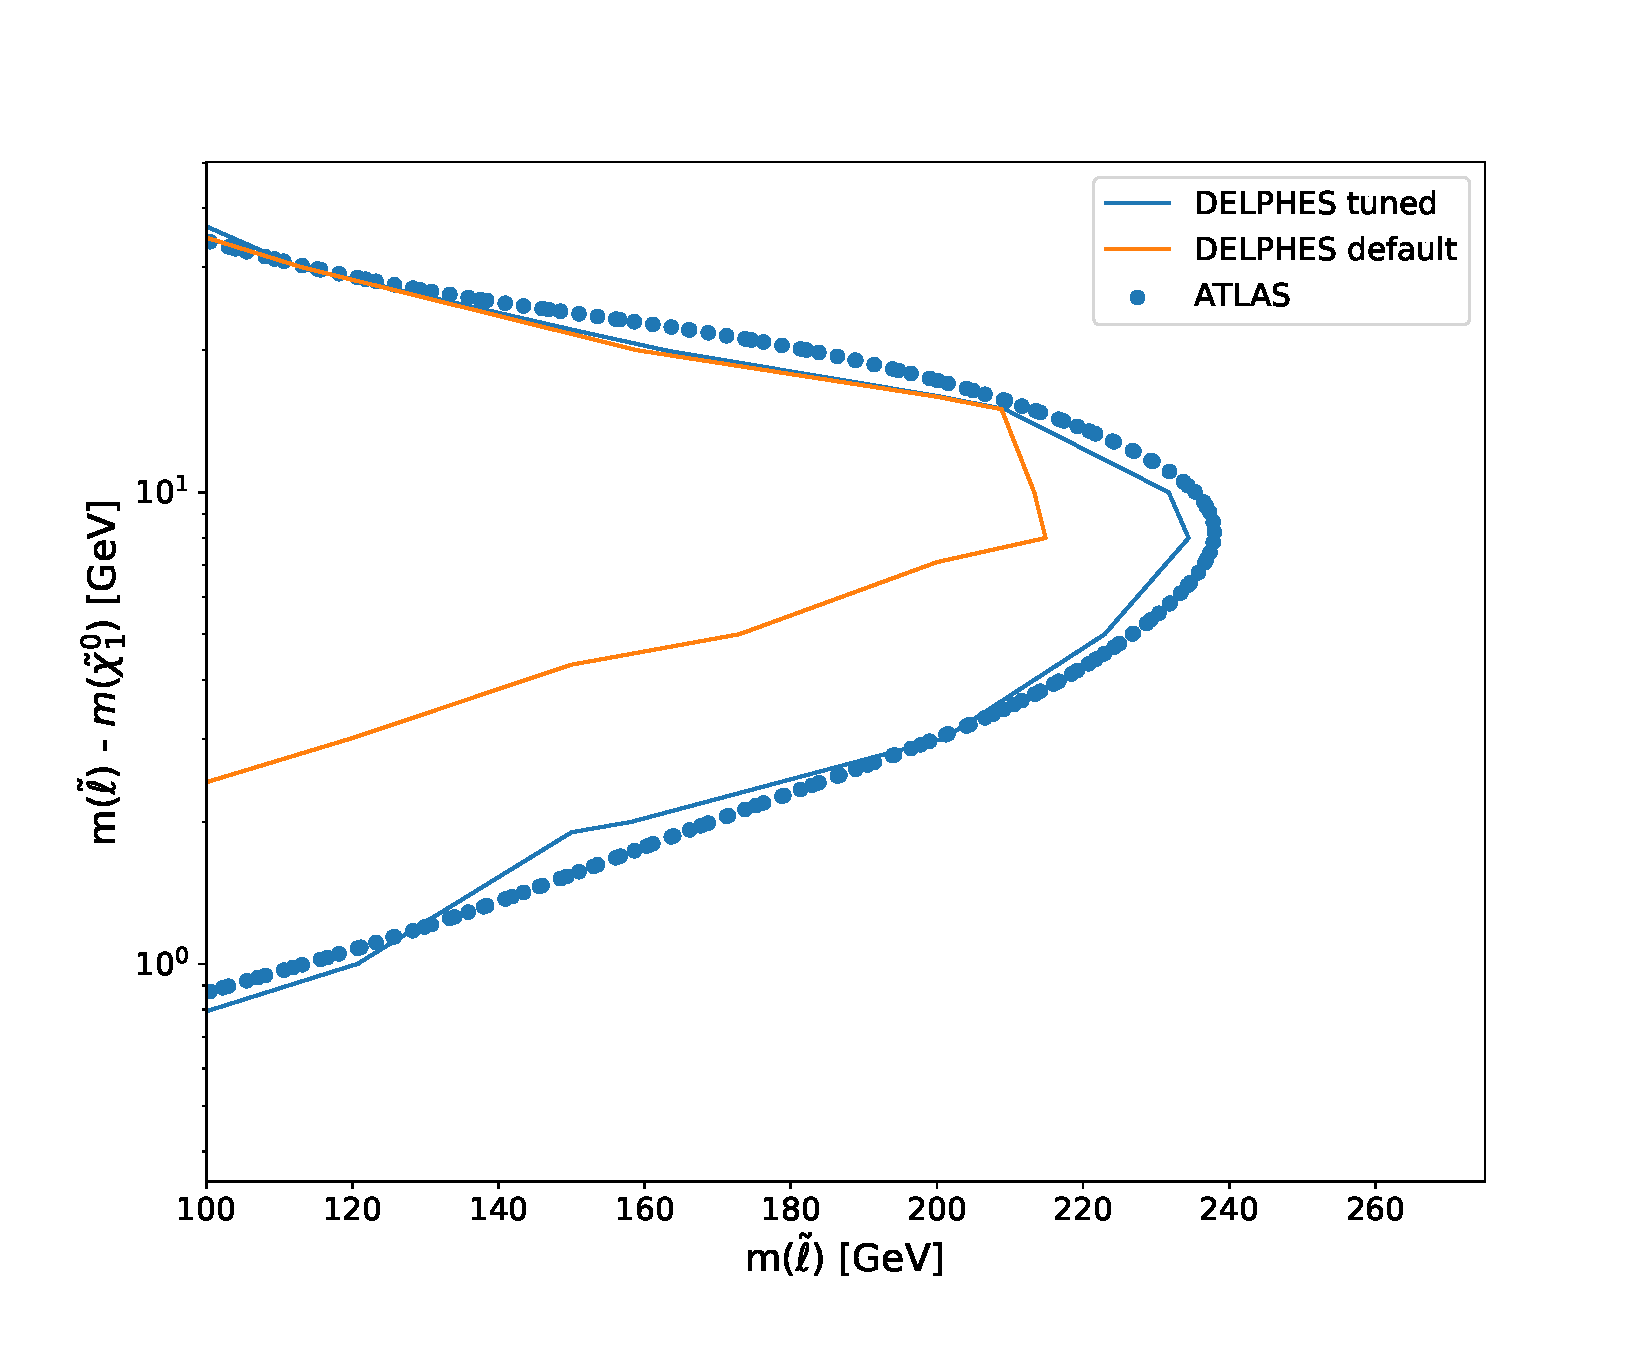
\includegraphics[width=0.5\textwidth]{{./figures/SleptonBino}}         %% examples/mapyde/SleptonBino_contours.ipynb
	\caption{Constraints on the slepton-bino model from the ATLAS paper~\cite{ATLAS:2019lng} (blue dots), from \mapyde{} before tuning the \delphes{} lepton efficiencies (orange solid), and from \mapyde{} after tuning (blue solid).}
	\label{fig:SleptonBino}
\end{figure}

With the framework tuned to the ATLAS response for compressed SUSY events, we now use \mapyde{} to assess the sensitivity of the ATLAS search to a new model.  We consider a \enquote{slepton-wino-bino} simplified model, where a light slepton decays with 100\% branching ratio to a wino-like \chitz{} NLSP and a SM charged lepton, with the \chitz{} decaying to a \chioz{} and two soft fermions, as illustrated in~\Cref{fig:feynman:slepton_wino_bino}. In order to reconstruct a lepton to be selected by the analysis, the slepton can decay either $\slepton\to\chitz$ or $\slepton\to\chiopm$ as illustrated in~\Cref{fig:feynman:slepton_decays}. However, the cross-section for electroweakly-produced SUSY would be further reduced by the branching ratio of the $W^\pm$/$Z^0$ making the \chiopm{}-mediated diagrams less useful for reinterpreation.  The \pt{} of the SM lepton will be largely determined by the slepton-\chitz{} mass gap, in contrast to the slepton-bino model where the lepton \pt{} is driven by the slepton-\chioz{} splitting.

\begin{figure}
	\centering
	\subfloat[neutralino-mediated]{\includegraphics[width=0.3\textwidth]{{./figures/feynman/output/slepton_decay_ch20}}}\hspace{2cm}
	\subfloat[chargino-mediated]{\includegraphics[width=0.3\textwidth]{{./figures/feynman/output/slepton_decay_ch1pm}}}
	\caption{Feynman diagrams of possible slepton decays via either (a) $\chitz$ or (b) $\chiopm$.}
	\label{fig:feynman:slepton_decays}
\end{figure}

We parameterize the model in terms of the slepton mass, the slepton-\chioz{} mass gap, and the \chitz-\chioz mass gap, to allow us to display the model constraints in the same plane as the slepton-bino results from ATLAS.  The resulting constraints (both expected and observed) are shown in~\Cref{fig:SleptonWinoBino} for a range of \chitz-\chioz{} splittings.  At small splittings the results resemble those of the slepton-bino model, since the \chitz{} is nearly degenerate with the \chioz{} leading to virtually no kinematic difference arising from the secondary decay of the \chitz.  By contrast, for large \chitz-\chioz{} splittings, given the requirement that the slepton must decay through a \chitz, the constrained parameter space is only at larger slepton-\chioz splittings, and covers a smaller range in slepton masses due to small slepton-\chitz{} splitting leading to softer SM leptons and lower lepton efficiencies.

\begin{figure}
	\centering
	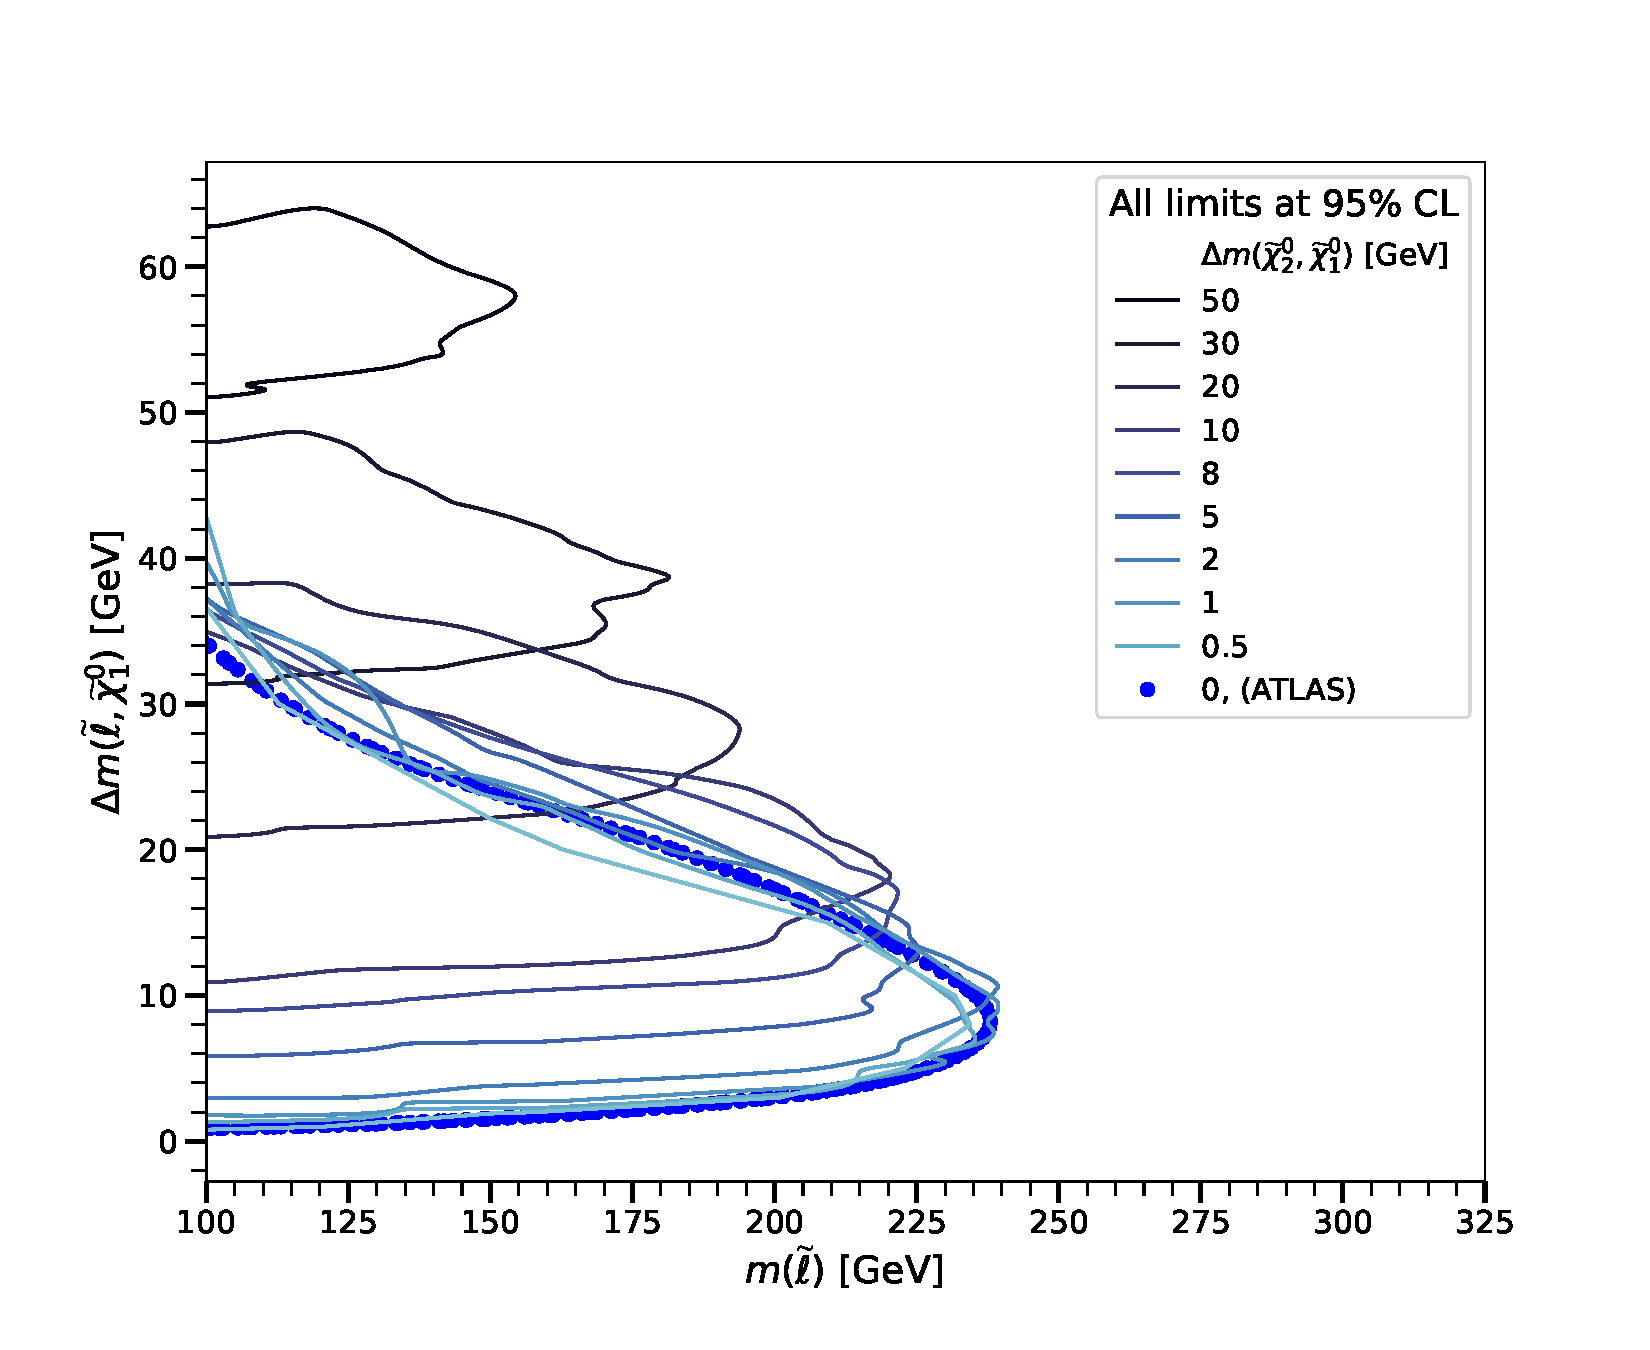
\includegraphics[width=0.48\textwidth]{{./figures/SleptonWinoBino_exp}}     %% examples/mapyde/SleptonWinoBino_contours.ipynb
	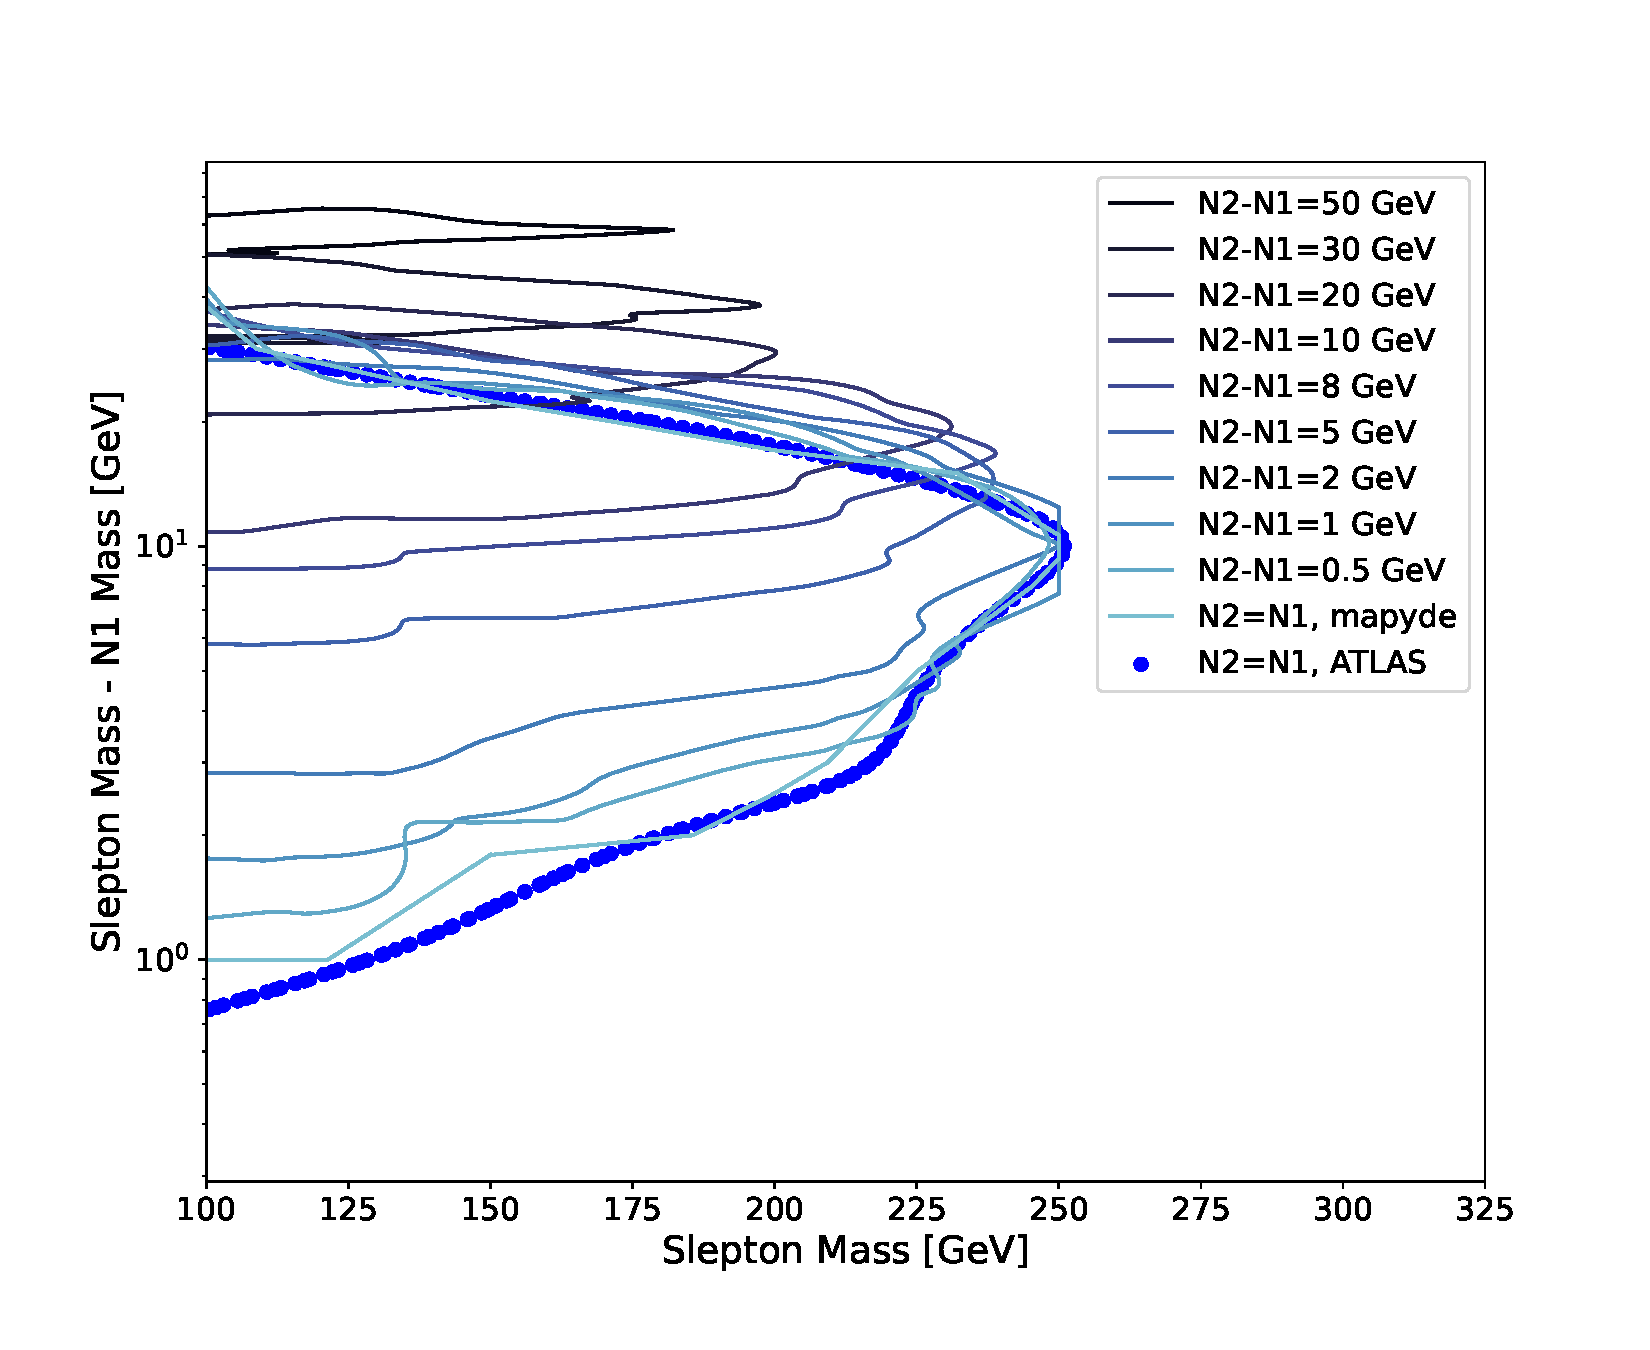
\includegraphics[width=0.48\textwidth]{{./figures/SleptonWinoBino_obs}}     %% examples/mapyde/SleptonWinoBino_contours.ipynb
	\caption{Expected (left) and observed (right) constraints on the slepton-wino-bino model.  The model is parameterized by the slepton mass, the slepton-\chioz{} mass splitting, and the \chitz-\chioz{} splitting, and compared against the slepton-bino results from Ref.~\cite{ATLAS:2019lng}.}
	\label{fig:SleptonWinoBino}
\end{figure}

This class of models, while being less \enquote{simplified} than the slepton-bino model traditionally studied by LHC experiments, includes models that nominally escape constraint by both existing slepton-bino searches as well as direct searches for electroweakinos.  In particular, the wino-bino constraints reported in Ref.~\cite{ATLAS:2019lng} constrain electroweakinos with \chitz-\chioz{} splittings as low as 1 GeV only for electroweakino masses near 100 GeV, while in the slepton-wino-bino model we can exclude models with 1 GeV \chitz-\chioz{} splittings up to \chioz{} masses of over 200 GeV.

\subsection{Compressed Electroweakinos}
\label{ssec:compressed-electroweakinos}

The ATLAS search for compressed electroweakinos considered two different simplified models: one with \enquote{pure} Higgsino-like \chitz, \chiopm, and \chioz{} states, and another with wino-like \chitz/\chiopm{} and bino-like \chioz.  We focus on the Higgsino model to validate the \mapyde{} output.  Following a procedure similar to the validation of the ATLAS slepton-bino results described above, we generate a grid of Higgsino model points to reproduce the Higgsino results.  The \mapyde{} electroweakino samples uses the same $k$-factor and lepton efficiencies as the slepton search.  The comparison between the \mapyde{} and ATLAS results is shown in~\Cref{fig:Higgsino}, where the \mapyde{} exclusion contour provides somewhat more coverage than the corresponding ATLAS contour, in contrast to the slepton-bino validation where the \mapyde{} results were slightly weaker than ATLAS.

\begin{figure}
	\centering
	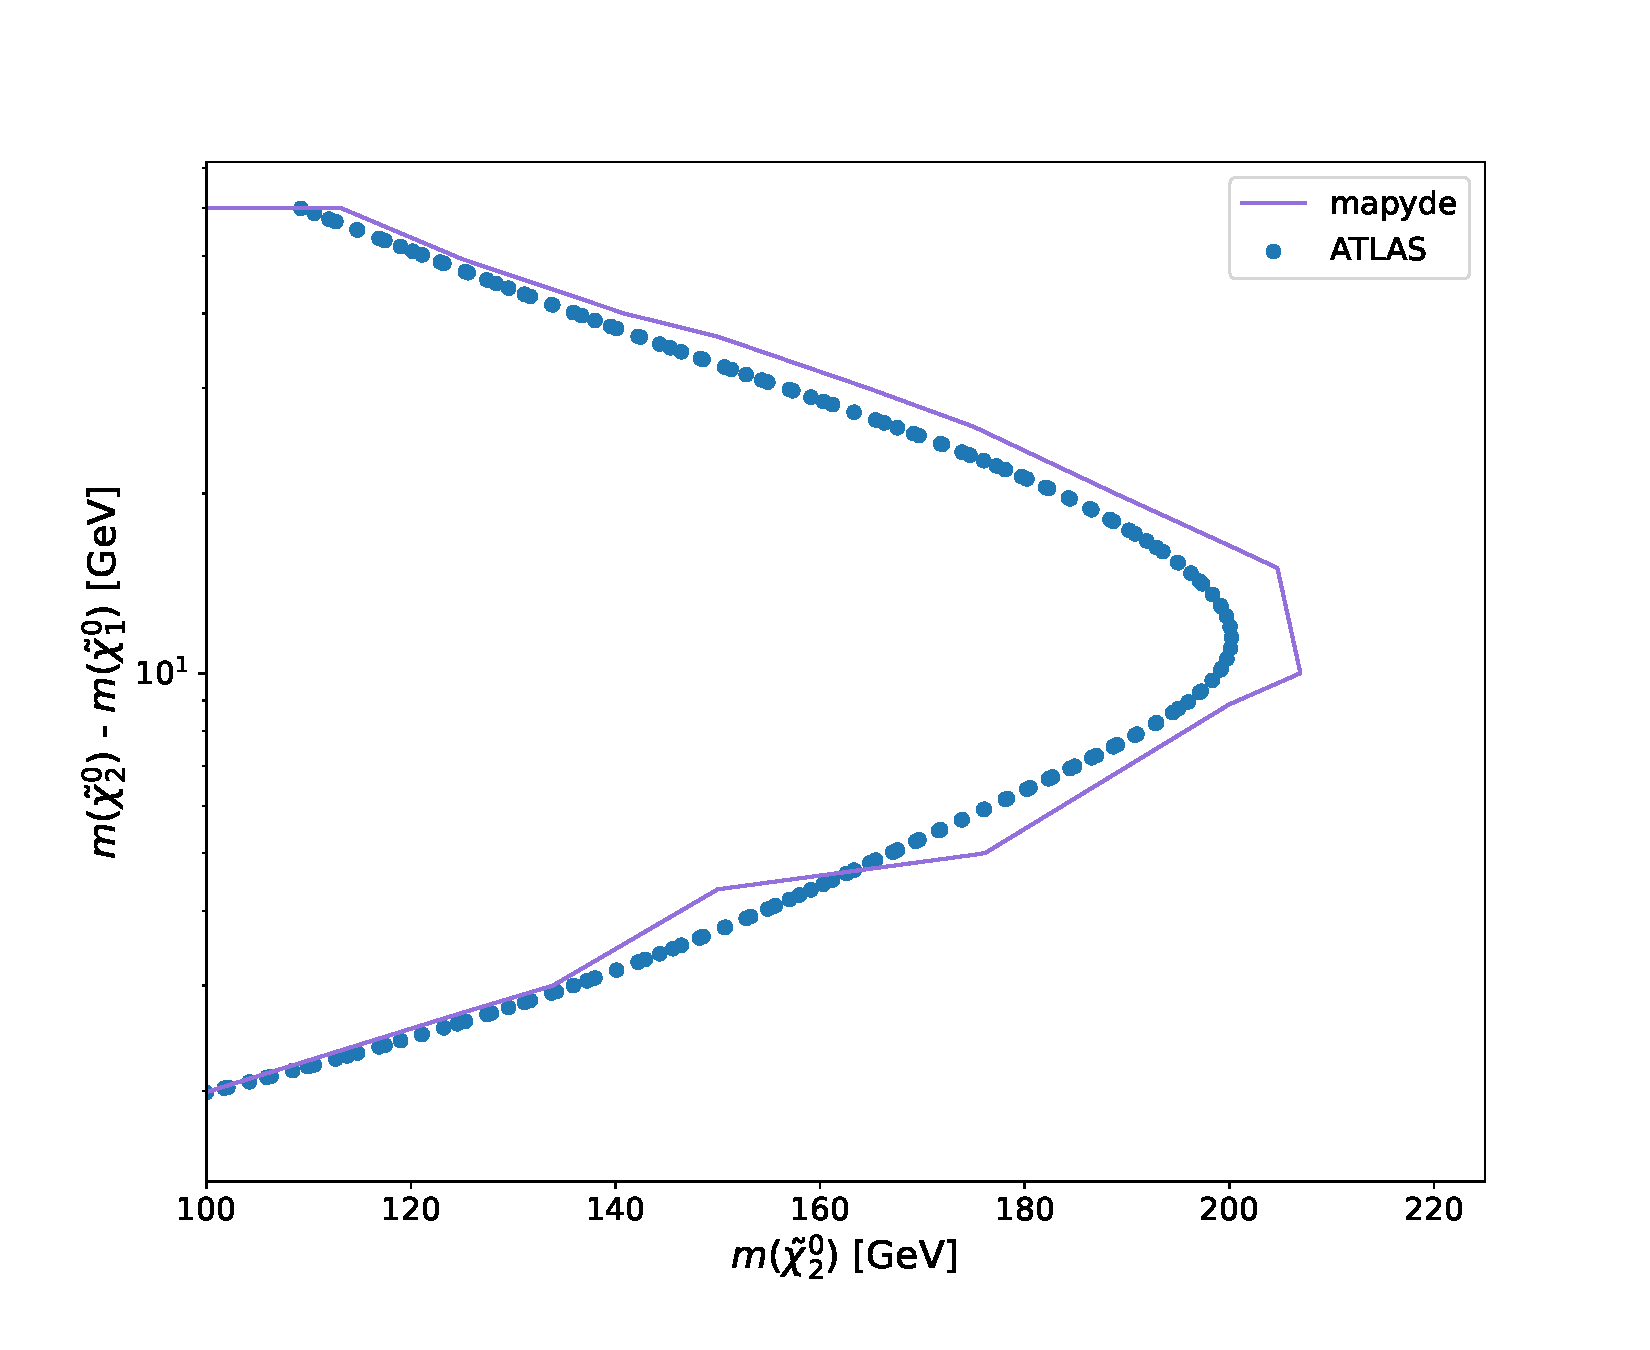
\includegraphics[width=0.5\textwidth]{{./figures/Higgsino}}         %% examples/mapyde/EWKino_contours.ipynb
	\caption{Constraints on the \enquote{pure Higgsino} simplified model from ATLAS (blue dots) and \mapyde{} (blue solid).}
	\label{fig:Higgsino}
\end{figure}

\begin{figure}
	\centering
	\subfloat[one-step]{\includegraphics[width=0.3\textwidth]{{./figures/feynman/output/ewkino_onestep}}}\hspace{2cm}
	\subfloat[two-step]{\includegraphics[width=0.3\textwidth]{{./figures/feynman/output/ewkino_twostep}}}
	\caption{Example feynman diagrams of possible electroweakino decays with (a) $\chitpm\to\chioz$ and (b) $\chitpm\to\chitz$. Note: in both cases above, the $W$-boson comes from $\chitpm$.}
	\label{fig:feynman:ewkinos}
\end{figure}

We next use \mapyde{} to assess the ATLAS sensitivity to SUSY models in which $M_1$, $M_2$, and $\mu$ are all relatively low, leading to \enquote{wino-bino-higgsino} models that have potentially rich phenomenologies. Some example models we are exploring the sensitivity to are illustrated in~\Cref{fig:feynman:ewkinos}. We use a pMSSM scanning tool (\easyscanhep~\cite{easyscanhep,Han:2016gvr}) to generate particle spectra for models with $M_1$, $M_2$, and $\mu$ ranging from -500 GeV to 500 GeV, sampled with flat priors, defined in~\Cref{lst:easyscanini}.  Particle masses are calculated using \spheno~\cite{Porod:2003um,Porod:2011nf} and stored in the SUSY Les Houches Accord (SLHA) format~\cite{Allanach:2008qq}.  Additional tools are run as described in~\Cref{sec:easyscan-hep-configuration}.  From this sample we select (\Cref{lst:mask}) 81 models satisfying $m(\chioz) > 100$ GeV, $m(\chithz)<300$ GeV, and $(m(\chithz)-m(\chioz))<50$ GeV for further study.  The SLHA records for these models are used as inputs for event generation, simulation, and analysis in \mapyde.  Branching ratios for electroweakino decays are taken directly from the \spheno{} output, with a constant $k$-factor of 1.2 applied to all samples.

\begin{listing}[H]
	\begin{minted}[frame=single,framesep=2mm]{python}
(SP_m_h!=-1) & (SPfh_m_h!=-1) & (MO_Omega!=-1) # spheno, feynhiggs, and micromegas ok
  & (SI_BR_Bs_to_mumu!=-1) & (GM2_gmuon!=-1) # superiso and gm2calc ok
  & (SP_m_chi_10>100) & (abs(SP_m_chi_30)<300) # N1 > 100 GeV, N3 < 300 GeV
  & ((abs(SP_m_chi_30)-abs(SP_m_chi_10))<50) # m(N3, N1) < 50 GeV
  \end{minted}
	\caption{The mask used to define the selection of models for assessing the ATLAS sensitivity to Higgsino-Wino models.}
	\label{lst:mask}
\end{listing}


The ATLAS constraints on the wino-bino-higgsino model scan are parameterized in terms of the mass of the \chitz and the mass difference $\Delta m=m(\chitz)-m(\chioz)$, to facilitate comparisons with the pure-Higgsino constraints from ATLAS.  The models under study are binned in a course grid in the $\Delta m$ vs $m(\chitz)$ plane, and the fraction of excluded models is calculated within each bin.  The expected and observed constraints on these models are shown in~\Cref{fig:EWKino_pmssm}, with the ATLAS Higgsino results overlaid for comparison.  In general the pMSSM points under study are more constrained than those of a pure-Higgsino model at larger mass splittings, likely due to the presence of the additional \chithz{} and its own decay to final states similar to that of the \chitz.

\begin{figure}
	\centering
	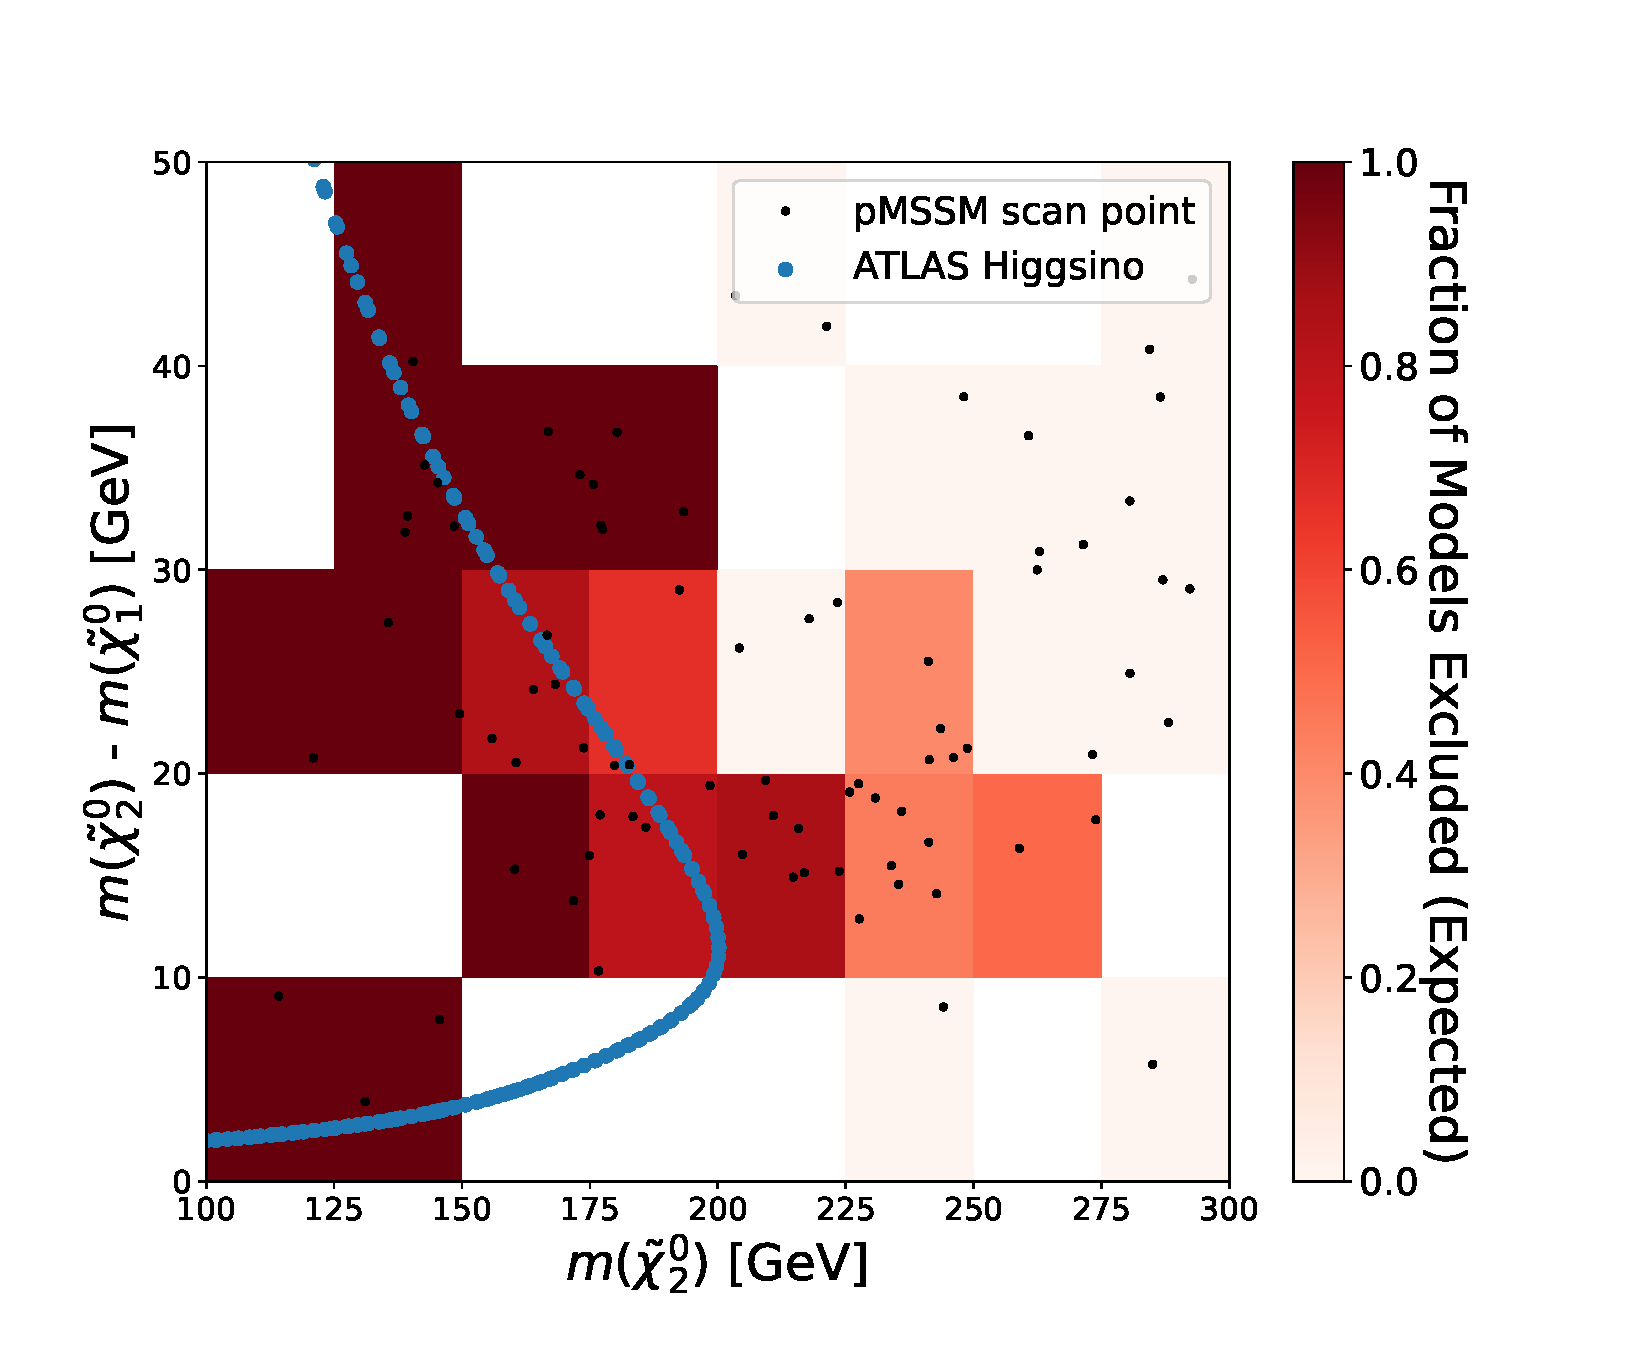
\includegraphics[width=0.48\textwidth]{{./figures/EWKino_pmssm_exp}}   %% examples/mapyde/WinoHiggsino_pmssm_contours.ipynb
	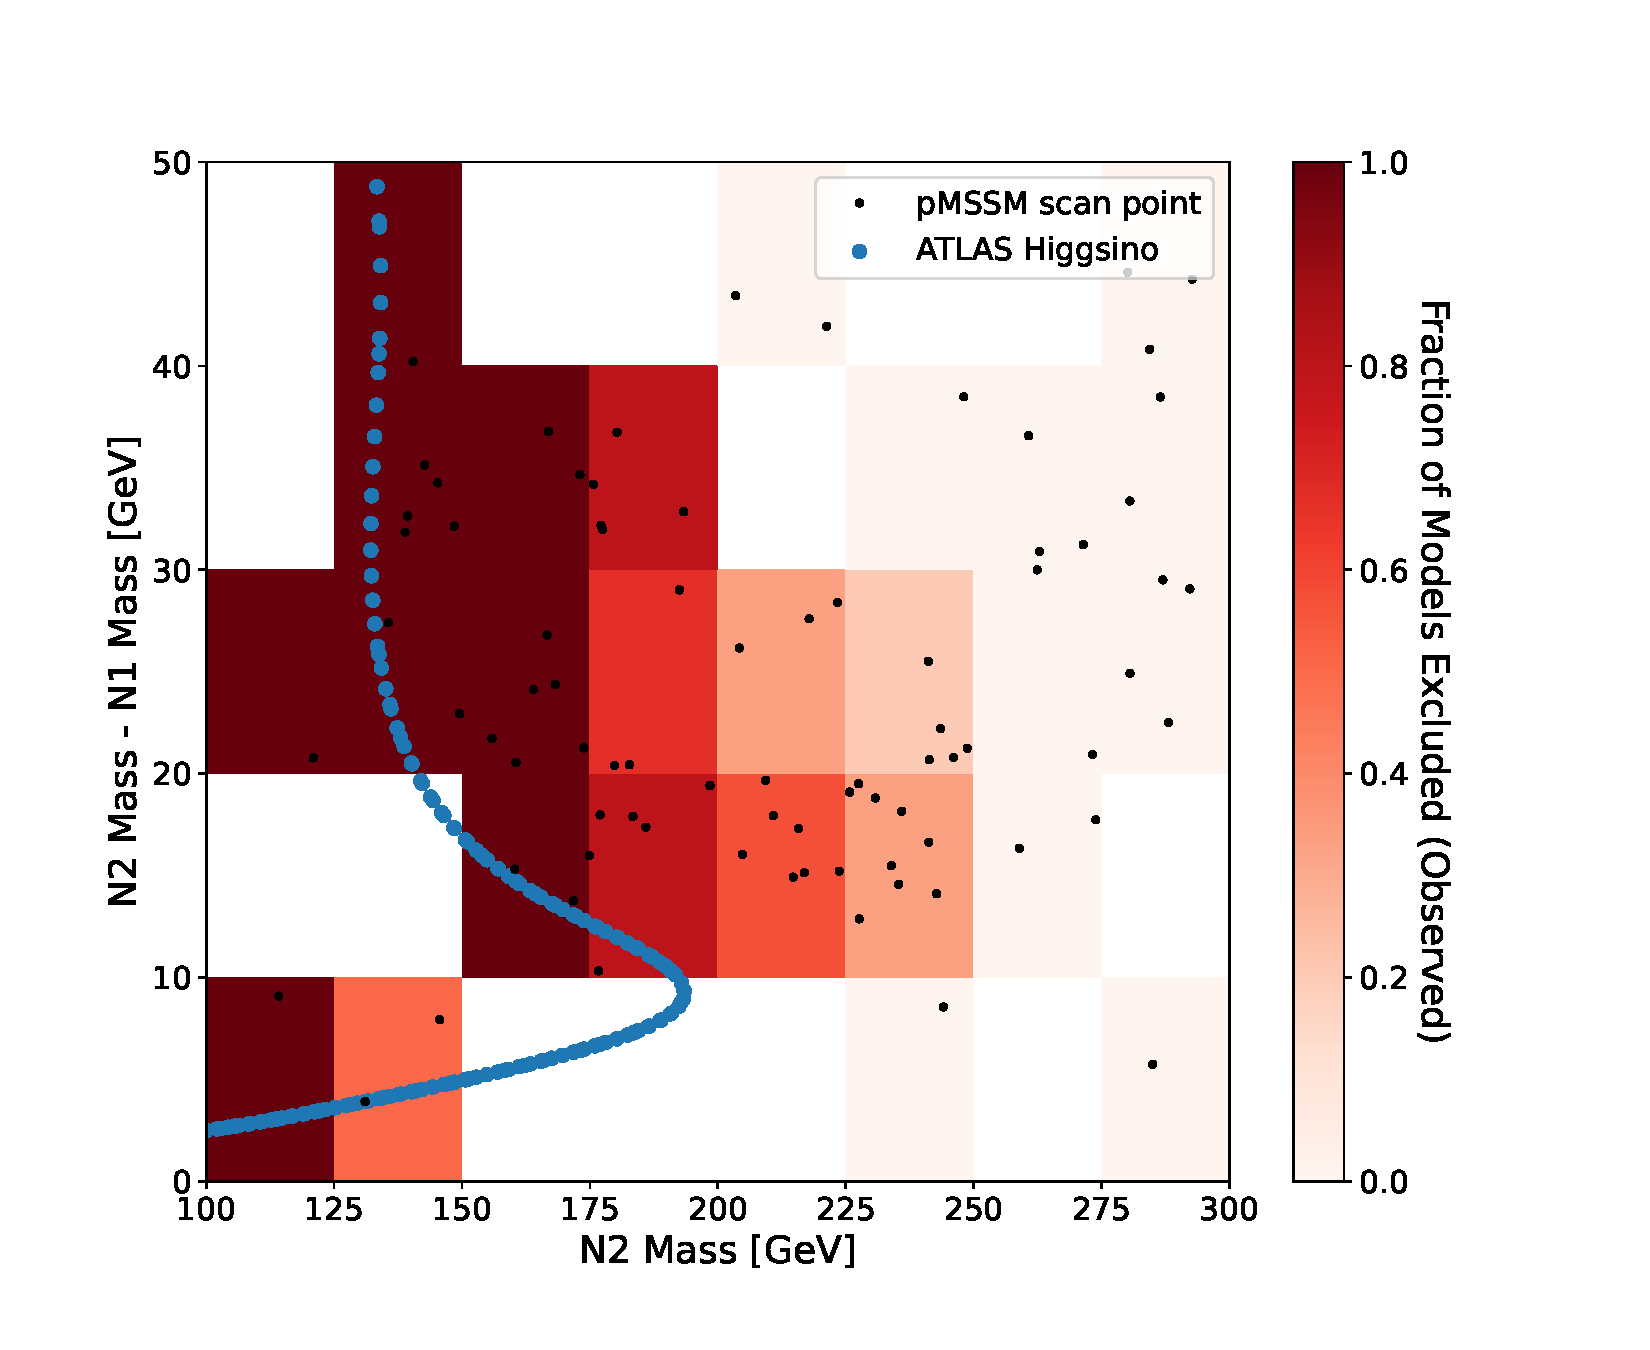
\includegraphics[width=0.48\textwidth]{{./figures/EWKino_pmssm_obs}}   %% examples/mapyde/WinoHiggsino_pmssm_contours.ipynb
	\caption{Expected (left) and observed (right) constraints on wino-bino-higgsino models containing three light neutralinos.  Black dots represent the specific model points used to calculate the fraction of excluded models within a bin, shown in color.  White bins contain no models from the current scan.  Results from an ATLAS search for pure Higgsinos are overlaid in blue dots.}
	\label{fig:EWKino_pmssm}
\end{figure}

\section{Conclusion}
\label{sec:conclusion}

We have presented \mapyde{}, shown some reinterpretations, and we're done.

\printbibliography

\appendix

\section{EasyScan\_HEP Configuration}
\label{sec:easyscan-hep-configuration}

We used an \easyscanhep \texttt{ini} configuration file that defined the scan ranges in~\Cref{lst:easyscanini} as well as additional programs to run, described in the text above. The specific versions used are:

\begin{itemize}
	\item \easyscanhep{} (\texttt{v1.0.0}): pMSSM scanning and program control~\cite{easyscanhep,Han:2016gvr}
	\item \spheno{} (\texttt{v4.0.4}): spectrum generator~\cite{Porod:2003um,Porod:2011nf}
	\item \feynhiggs{} (\texttt{v2.16.0}): Higgs mass calculation~\cite{Bahl:2018qog,Bahl:2017aev,Bahl:2016brp,Hahn:2013ria,Frank:2006yh,Degrassi:2002fi,Heinemeyer:1998np,Heinemeyer:1998yj}
	\item \micromegas{} (\texttt{v5.2.1}): Dark Matter calculations (e.g., relic density)~\cite{Belanger:2020gnr}
	\item \superiso{} (\texttt{v4.0}): Flavor Physics observables~\cite{Arbey:2018msw}
	\item \gmtwocalc{} (\texttt{v2.0.0}): $g-2$ calculation~\cite{Athron:2015rva,Athron:2021evk}
\end{itemize}

\begin{listing}[H]
	\begin{minted}[frame=single,framesep=2mm]{ini}
[scan]
Scan method:       random
#                  ID     Prior  Min    MAX
Input parametes:   tanb,  Flat,  1,     60
                   M_1,   Flat,  2000,  2000
                   M_2,   Flat,  -500,  500
                   M_3,   Flat,  2000,  2000
                   AT,    Flat,  2000,  2000
                   Ab,    Flat,  2000,  2000
                   Atau,  Flat,  2000,  2000
                   MU,    Flat,  -500,  500
                   mA,    Flat,  2000,  2000
                   meL,   Flat,  2000,  2000
                   mtauL, Flat,  2000,  2000
                   meR,   Flat,  2000,  2000
                   mtauR, Flat,  2000,  2000
                   mqL1,  Flat,  2000,  2000
                   mqL3,  Flat,  2000,  2000
                   muR,   Flat,  2000,  2000
                   mtR,   Flat,  2000,  2000
                   mdR,   Flat,  2000,  2000
                   mbR,   Flat,  2000,  2000
  \end{minted}
	\caption{A portion of the \texttt{easyscan.ini} configuration defining the random sampling for the electroweakinos scan.}
	\label{lst:easyscanini}
\end{listing}


\end{document}
